\documentclass[letterpaper,12pt,fleqn,reqno]{amsart}

\usepackage[margin=1in]{geometry}
\usepackage{url}
\usepackage{tikz}
\usepackage{graphicx}

\theoremstyle{plain}
\newtheorem{theorem}{Theorem}[section]
\newtheorem{lemma}[theorem]{Lemma}
\newtheorem{corollary}[theorem]{Corollary}
\newtheorem{definition}[theorem]{Definition}
\newtheorem{properties}[theorem]{Properties}

\newcommand{\N}{\mathbb{N}}
\newcommand{\Z}{\mathbb{Z}}
\newcommand{\R}{\mathbb{R}}
\newcommand{\vp}{\varphi}
\renewcommand{\d}{\delta}
\newcommand{\e}{\epsilon}
\renewcommand{\k}{\kappa}
\renewcommand{\o}{\theta}
\newcommand{\Lop}{L^1[-\pi,\pi]}
\newcommand{\Lor}{L^1(\R)}
\newcommand{\Ltp}{L^2[-\pi,\pi]}

\newcommand{\abs}[1]{\left|#1\right|}
\newcommand{\norm}[1]{\left\|#1\right\|}
\newcommand{\inner}[1]{\left<#1\right>}
\newcommand{\conj}[1]{\overline{#1}}

\newcommand{\Fej}{Fej\'{e}r\ }
\newcommand{\Ces}{Ces\'{a}ro\ }

\everymath{\displaystyle}

\begin{document}

\title{A Complete Orthonormal Sequence for $\Ltp$}

\author{Jeffery Cavallaro}

\address{Department of Mathematics, San Jos\'e State University, San
  Jos\'e, CA 95192-0103}

\email{jeffery.cavallaro@sjsu.edu}

\thanks{\textsc{Math 231B: Functional Analysis}}

\date{\today}

\begin{abstract}
  The goal of this paper is to prove that the sequence $(\vp_n)$, where
  $\vp_n(x)=\frac{1}{\sqrt{2\pi}}e^{inx}$, is a bi-infinite complete orthonormal
  sequence in $\Ltp$. The fact that $(\vp_n)$ is orthonormal is fairly
  straightforward and is proved in the normal way using inner products.
  The fact that $(\vp_n)$ is complete is a bit more complicated. The method
  used here is to first use H\"{o}lder's inequality to show that if $f\in\Ltp$
  then $f\in\Lop$. Next, the \Fej summability kernel is used to show that
  for all $f\in\Lop$, if $\hat{f}(n)=\inner{f,\vp_n}_{L_2}=0$ for all $n\in\Z$
  then $f\equiv0$ a.e., which is sufficient to conclude that $(\vp_n)$ is
  complete in $\Ltp$.
\end{abstract}

\maketitle

\section{Introduction}

The rise of the relatively new fields of electrical engineering and signal
analysis during the late $19^{th}$ and early $20^{th}$ centuries motivated the
mathematicians of the time to develop new theoretical frameworks for the
growing fields. One such leader was the Jewish-Hungarian mathematician
Lip\'{o}t \Fej (1880--1959). \Fej made major contributions to the theory
of harmonic analysis, as well as being advisor and mentor to many future giants
in the field, including: John Von Neumann, Paul Erd\"{o}s, and George P\'{o}lya.

Since many physical phenomena can be expressed as harmonic functions in
$L^2[-\pi,\pi]$, it is important to have a theoretically sound orthonormal
basis for the space. The existence of such a basis facilitates the solutions
to both theoretical and practical problems, especially in the areas of
waveform analysis. A candidate for such a basis is the Dirichlet sequence:
$(\vp_n)$, where $\vp_n(t)=\frac{1}{\sqrt{2\pi}}e^{int}$. It is fairly easy
to prove the orthonormality of this sequence; however, its completeness is a
bit more complicated and requires the use of so-called summability kernels.
The summability kernel that will be used in this proof is attributed to
\Fej. Indeed, the use of summability kernels is an important tool in
analysis.

\section{Orthonormality}

The first order of business is to establish the orthonormal nature of the
sequence $(\vp_n)$ in $\Ltp$, where $\vp_n(x)=\frac{1}{\sqrt{2\pi}}e^{inx}$.

The following lemma is helpful both here and later:

\begin{lemma}
  \label{lem:e}
  $\int_{-\pi}^{\pi}e^{inx}dx=\begin{cases}
  2\pi, & n=0 \\
  0, & n\in\Z-\{0\}
  \end{cases}$
\end{lemma}

\begin{proof}
  Assume $n\in\Z$.

  \begin{description}
  \item[Case 1] $n=0$
    \begin{eqnarray*}
      \int_{-\pi}^{\pi}e^{i0x}dx &=& \int_{-\pi}^{\pi}dx\quad=\quad2\pi
    \end{eqnarray*}

  \item[Case 2] $n\ne0$
    \begin{eqnarray*}
      \int_{-\pi}^{\pi}e^{inx}dx &=&
      \left.\frac{1}{in}e^{inx}\right|_{-\pi}^{\pi} \\
      &=& \frac{1}{in}(e^{in\pi}-e^{-in\pi}) \\
      &=& \frac{2}{n}\left(\frac{e^{in\pi}-e^{-in\pi}}{2i}\right) \\
      &=& \frac{2}{n}\sin(n\pi) \\
      &=& 0
    \end{eqnarray*}
  \end{description}
\end{proof}

The following corollary follows directly from the above lemma:

\begin{corollary}
  $\int_{-\pi}^{\pi}\vp_n(x)dx=\begin{cases}
  \sqrt{2\pi}, & n=0 \\
  0, & n\in\Z-\{0\}
  \end{cases}$
\end{corollary}

\begin{proof}
  Assume $n\in\Z$.

  \begin{description}
  \item[Case 1] $n=0$
    \[\int_{-\pi}^{\pi}\vp_0(x)dx=\frac{1}{\sqrt{2\pi}}\int_{-\pi}^{\pi}e^{i0x}dx=
    \frac{1}{\sqrt{2\pi}}2\pi=\sqrt{2\pi}\]

  \item[Case 2] $n\ne0$
    \[\int_{-\pi}^{\pi}\vp_n(x)dx=\frac{1}{\sqrt{2\pi}}\int_{-\pi}^{\pi}e^{inx}dx=
    \frac{1}{\sqrt{2\pi}}\cdot0=0\]
  \end{description}
\end{proof}

And so orthonormality in $\Ltp$ follows easily:

\begin{theorem}
  $(\vp_n)$ is an orthonormal sequence in $\Ltp$.
\end{theorem}

\begin{proof}
  Assume $n,m\in\Z$

  \begin{description}
  \item[Case 1] $m=n$
    \begin{eqnarray*}
      \inner{\vp_n,\vp_n} &=& \int_{-\pi}^{\pi}\vp_n(x)\conj{\vp_n(x)}dx \\
      &=& \frac{1}{2\pi}\int_{-\pi}^{\pi}e^{inx}\conj{e^{inx}}dx \\
      &=& \frac{1}{2\pi}\int_{-\pi}^{\pi}e^{inx}e^{-inx}dx \\
      &=& \frac{1}{2\pi}\int_{-\pi}^{\pi}dx \\
      &=& \frac{1}{2\pi}2\pi \\
      &=& 1
    \end{eqnarray*}
    
  \item[Case 2] $m\ne n$
    \begin{eqnarray*}
      \inner{\vp_m,\vp_n} &=& \int_{-\pi}^{\pi}\vp_m(x)\conj{\vp_n(x)}dx \\
      &=& \frac{1}{2\pi}\int_{-\pi}^{\pi}e^{imx}\conj{e^{inx}}dx \\
      &=& \frac{1}{2\pi}\int_{-\pi}^{\pi}e^{imx}e^{-inx}dx \\
      &=& \frac{1}{2\pi}\int_{-\pi}^{\pi}e^{i(m-n)x}dx \\
      &=& \frac{1}{2\pi}\cdot0 \\
      &=& 0
    \end{eqnarray*}
  \end{description}
\end{proof}

\section{Convolution}

The proof will require the services of the \emph{convolution} binary operator
on $\Lop$. In order to get a feel for this operator, it is helpful to observe
its behavior in $\Lor$:
\begin{definition}[Convolution]
  Let $f,g\in\Lor$. The convolution of $f$ and $g$, denoted $f\star g$, is
  given by:
  \[(f\star g)(x)=\int_{-\infty}^{\infty}f(x-t)g(t)dt\]
\end{definition}
The first thing to note about this definition is that since $f\in\Lor$,
reflecting and translating $f$ does not affect its integrability over $\R$,
and thus $f\star g\in\Lor$ as well.

Next, consider what is happening from a function transformation standpoint:
\begin{enumerate}
\item Express $f$ and $g$ in terms of a dummy variable $t$.
\item Reflect $f(t)$ to get $f(-t)$.
\item As $x$ varies from $-\infty$ to $\infty$, the reflected $f(t)$ sweeps
  across $g(t)$.
\end{enumerate}
Therefore, for a given $x$, $(f\star g)(x)$ provides a weighted summation of
the intersection of $f(x-t)$ and $g(t)$.

For example, let $f(x)=g(x)$ be the unit rectangular pulse:
\[f(x)=\begin{cases}
1, & x\in[0,1] \\
0, & otherwise
\end{cases}\]
Note that for $x\notin(0,2)$ there is no overlap and thus $(f\star f)(x)=0$
(see Figure \ref{fig:conv:noover}).

\begin{figure}[ht]
  \begin{tikzpicture}[scale=2]
    \draw (-2,0) -- (5,0) node [right] {$t$};
    \draw (0,-1) -- (0,3/2);
    \draw [line width=1mm] (0,0) -- (0,1) -- (1,1) -- (1,0);
    \draw [line width=1mm] (3,0) -- (3,1) -- (4,1) -- (4,0);
    \node [below left] at (0,0) {$0$};
    \node [below] at (1,0) {$1$};
    \node [below] at (3,0) {$x-1$};
    \node [below] at (4,0) {$x$};
    \draw [dashed] (-2,1) -- (5,1);
    \node [above left] at (0,1) {$1$};
  \end{tikzpicture}
  \caption{Convolution with No Overlap}
  \label{fig:conv:noover}
\end{figure}

However, for $x\in(0,2)$ there is indeed overlap
(see Figure \ref{fig:conv:over}).

\begin{figure}[ht]
  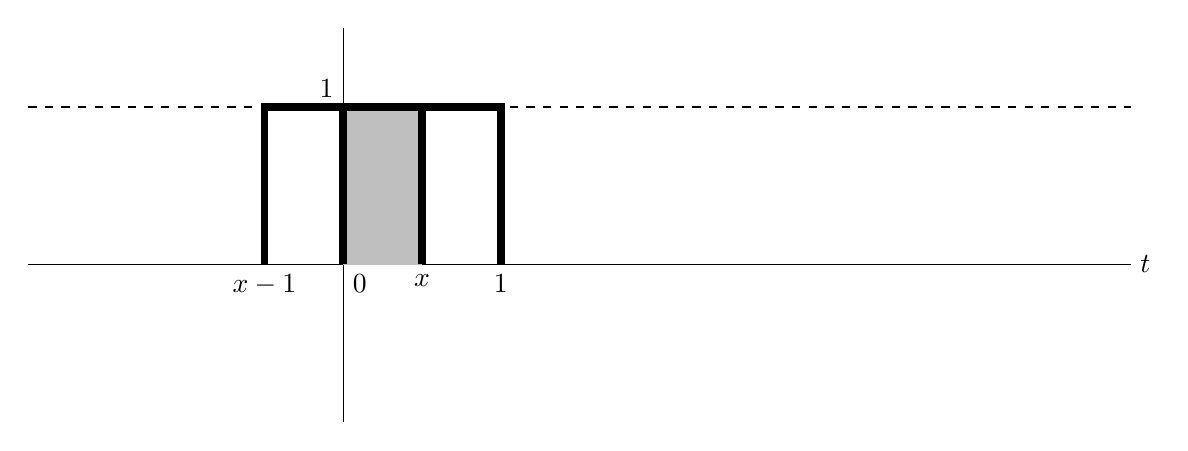
\begin{tikzpicture}[scale=2]
    \draw (-2,0) -- (5,0) node [right] {$t$};
    \draw (0,-1) -- (0,3/2);
    \draw [fill,color=lightgray] (0,0) rectangle (1/2,1);
    \draw [line width=1mm] (0,0) -- (0,1) -- (1,1) -- (1,0);
    \draw [line width=1mm] (-1/2,0) -- (-1/2,1) -- (1/2,1) -- (1/2,0);
    \node [below] at (-1/2,0) {$x-1$};
    \node [below right] at (0,0) {$0$};
    \node [below] at (1/2,0) {$x$};
    \node [below] at (1,0) {$1$};
    \draw [dashed] (-2,1) -- (5,1);
    \node [above left] at (0,1) {$1$};
  \end{tikzpicture}
  \caption{Convolution with Overlap}
  \label{fig:conv:over}
\end{figure}

Indeed, for this example, the area of overlap increases linearly for
$x\in[0,1]$, reaching its peak at $x=1$, and then decreases linearly for
$x\in[1,2]$. Therefore, the result is a triangular pulse of width $2$
(see Figure \ref{fig:conv:result}).

\begin{figure}[ht]
  \begin{tikzpicture}[scale=2]
    \draw (-2,0) -- (5,0) node [right] {$t$};
    \draw (0,-1) -- (0,3/2);
    \draw [line width=1mm] (0,0) -- (1,1) -- (2,0);
    \draw [dashed] (1,0) -- (1,1);
    \node [below left] at (0,0) {$0$};
    \node [below] at (1,0) {$1$};
    \node [below] at (2,0) {$2$};
    \draw [dashed] (-2,1) -- (5,1);
    \node [above left] at (0,1) {$1$};
  \end{tikzpicture}
  \caption{Convolution of Two Unit Rectangular Pulses}
  \label{fig:conv:result}
\end{figure}

Now, turning specifically to the interval $[-\pi,\pi]$, there is a one-to-one
correspondence between functions in $\Lop$ and $2\pi$-periodic functions in
$\Lor$. Thus, it will be convenient to use a slightly modified version of the
convolution operator:
\begin{definition}[Convolution on the Circle]
  Let $f,g\in\Lor$ be $2\pi$-periodic. Convolution on the circle is given by:
  \[(f\star g)(x)=\frac{1}{2\pi}\int_{-\pi}^{\pi}f(x-t)g(t)dt\]
\end{definition}
Note that this adjusted definition provides an average weighted value over
the circle.

Regardless of which definition is used, convolution is commutative.
\begin{theorem}
  Let $f,g\in\Lor$. Then:
  \[(f\star g)(x)=(g\star f)(x)\]
\end{theorem}

\begin{proof}
  Using the substitution $u=x-t$:
  \begin{eqnarray*}
    (f\star g)(x) &=& \int_{-\infty}^{\infty}f(x-t)g(t)dt \\
    &=& \int_{\infty}^{-\infty}f(u)g(x-u)(-du) \\
    &=& \int_{-\infty}^{\infty}f(u)g(x-u)du \\
    &=& \int_{-\infty}^{\infty}g(x-u)f(u)du \\
    &=& (g\star f)(x)
  \end{eqnarray*}
\end{proof}

\begin{theorem}
  Let $f,g\in\Lor$ such that $f$ and $g$ are $2\pi$-periodic. Then:
  \[(f\star g)(x)=(g\star f)(x)\]
  where convolution is on the circle.
\end{theorem}

\begin{proof}
  Using the substitution $u=x-t$:
  \begin{eqnarray*}
    (f\star g)(x) &=& \int_{-\pi}^{\pi}f(x-t)g(t)dt \\
    &=& \int_{x+\pi}^{x-\pi}f(u)g(x-u)(-du) \\
    &=& \int_{x-\pi}^{x+\pi}f(u)g(x-u)du \\
    &=& \int_{-\pi}^{\pi}g(x-u)f(u)du \\
    &=& (g\star f)(x)
  \end{eqnarray*}
\end{proof}
Of course, commutativity makes sense because the ``sweeping'' of either
function is relative.

\section{Summability Kernel}

The proof uses the notion of a \emph{summability} kernel to help show
convergence in a norm.

\begin{definition}[Summability Kernel]
  To say that a sequence $(\k_n)$ of $2\pi$-periodic continuous fuctions is
  a summability kernel means that $\k_n$ satisfies the following properties:
  \begin{enumerate}
  \item $\int_{-\pi}^{\pi}\k_n(t)dt=2\pi$
  \item $\int_{-\pi}^{\pi}\abs{\k_n(t)}dt\le M$ for some $M>0$ and all
    $n\in\N$
  \item $\int_{\d\le\abs{t}\le\pi}\abs{\k_n(t)}dt\to0$ for all $\d\in(0,\pi)$
  \end{enumerate}
\end{definition}
Note that the third property indicates that given a $\d>0$, for all $\e>0$
there exists an $n$ sufficiently large such:
\[2\pi(1-\e)<\int_{-\d}^{\d}\k_n(t)dt\le2\pi\]

The importance of summability kernels and convolution is embodied by the
following key theorem:

\begin{theorem}
  \label{thm:key}
  Let $(\k_n)$ be a summability kernel and let $f\in\Lop$:
  \[\norm{(k_n\star f)-f}_1\to 0\]
  In other words, $k_n\star f$ converges to $f$ in the $\Lop$ norm.
\end{theorem}

\begin{proof}
  From the first property:
  \begin{eqnarray*}
    \int_{-\pi}^{\pi}\k_n(t)dt &=& 2\pi \\
    \frac{1}{2\pi}\int_{-\pi}^{\pi}\k_n(t)dt &=& 1 \\
    f(x)\frac{1}{2\pi}\int_{-\pi}^{\pi}\k_n(t)dt &=& f(x) \\
    \frac{1}{2\pi}\int_{-\pi}^{\pi}\k_n(t)f(x)dt &=& f(x)
  \end{eqnarray*}
  And so:
  \begin{eqnarray*}
    (\k_n\star f)(x)-f(x) &=&
    \frac{1}{2\pi}\int_{-\pi}^{\pi}\k_n(t)f(x-t)dt-
    \frac{1}{2\pi}\int_{-\pi}^{\pi}\k_n(t)f(x)dt \\
    &=& \frac{1}{2\pi}\int_{-\pi}^{\pi}\k_n(t)[f(x-t)-f(x)]dt
  \end{eqnarray*}
  Now construct the $\Lop$ norm:
  \begin{eqnarray*}
    \int_{-\pi}^{\pi}\abs{(\k_n\star f)(x)-f(x)}dx &=& \int_{-\pi}^{\pi}
    \abs{\frac{1}{2\pi}\int_{-\pi}^{\pi}\k_n(t)[f(x-t)-f(x)]dt}dx \\
  \end{eqnarray*}
  Now, assume $\d\in(0,\pi)$:
  \begin{eqnarray*}
    \norm{(\k_n\star f)-f}_1 &=& \int_{-\pi}^{\pi}
    \abs{\frac{1}{2\pi}\left\{\int_{-\d}^{\d}\k_n(t)[f(x-t)-f(x)]dt+
      \int_{\d\le\abs{t}\le\pi}\k_n(t)[f(x-t)-f(x)]dt\right\}}dx \\
    &\le& \frac{1}{2\pi}\int_{-\pi}^{\pi}
    \left\{\abs{\int_{-\d}^{\d}\k_n(t)[f(x-t)-f(x)]dt}+
    \abs{\int_{\d\le\abs{t}\le\pi}\k_n(t)[f(x-t)-f(x)]dt}\right\}dx \\
    &=& \frac{1}{2\pi}\int_{-\pi}^{\pi}
    \abs{\int_{-\d}^{\d}\k_n(t)[f(x-t)-f(x)]dt}dx \\
    &+& \frac{1}{2\pi}\int_{-\pi}^{\pi}
    \abs{\int_{\d\le\abs{t}\le\pi}\k_n(t)[f(x-t)-f(x)]dt}dx \\
    &\le& \frac{1}{2\pi}\int_{-\pi}^{\pi}
    \int_{-\d}^{\d}\abs{\k_n(t)[f(x-t)-f(x)]}dtdx \\
    &+& \frac{1}{2\pi}\int_{-\pi}^{\pi}
    \int_{\d\le\abs{t}\le\pi}\abs{\k_n(t)[f(x-t)-f(x)]}dtdx \\
  \end{eqnarray*}
  Assume $\e>0$.

  Focusing on the first term in the last sum:
  \begin{eqnarray*}
    \frac{1}{2\pi}\int_{-\pi}^{\pi}
    \int_{-\d}^{\d}\abs{\k_n(t)[f(x-t)-f(x)]}dtdx &=&
    \frac{1}{2\pi}\int_{-\pi}^{\pi}
    \int_{-\d}^{\d}\abs{\k_n(t)}\abs{f(x-t)-f(x)}dtdx \\
    &\le& \frac{1}{2\pi}\left[
      \max_{\abs{t}\le\d}\int_{-\pi}^{\pi}\abs{f(x-t)-f(x)}dx\right]
    \int_{-\d}^{\d}\abs{\k_n(t)}dt \\
    &\le& \frac{1}{2\pi}\left[
      \max_{\abs{t}\le\d}\int_{-\pi}^{\pi}\abs{f(x-t)-f(x)}dx\right]
    \int_{-\pi}^{\pi}\abs{\k_n(t)}dt
  \end{eqnarray*}
  As $t\to0$, the translated function $f(x-t)\to f(x)$ and
  $\int_{-\pi}^{\pi}\abs{f(x-t)-f(x)}dx\to0$. Furthermore,
  $\int_{-\pi}^{\pi}\abs{\k_n(t)}dt$ is bounded by the second property. Thus, it
  is possible to select $\d$ small enough such that:
  \[\frac{1}{2\pi}\int_{-\pi}^{\pi}
  \int_{-\d}^{\d}\abs{\k_n(t)[f(x-t)-f(x)]}dtdx<\frac{\e}{2}\]
  for all $n\in\N$.

  Focusing on the second term:
  \begin{eqnarray*}
    \frac{1}{2\pi}\int_{-\pi}^{\pi}
    \int_{\d\le\abs{t}\le\pi}\abs{\k_n(t)[f(x-t)-f(x)]}dtdx &=&
    \frac{1}{2\pi}\int_{-\pi}^{\pi}
    \int_{\d\le\abs{t}\le\pi}\abs{\k_n(t)}\abs{f(x-t)-f(x)}dtdx \\
    &\le& \frac{1}{2\pi}\left[
      \max_{\d\le\abs{t}\le\pi}\int_{-\pi}^{\pi}\abs{f(x-t)-f(x)}dx\right]
    \int_{\d\le\abs{t}\le\pi}\abs{\k_n(t)}dt \\
  \end{eqnarray*}
  But note that:
  \begin{eqnarray*}
    \int_{-\pi}^{\pi}\abs{f(x-t)-f(x)}dx &\le&
    \int_{-\pi}^{\pi}[\abs{f(x-t)}+\abs{f(x)}]dx \\
    &=& \int_{-\pi}^{\pi}\abs{f(x-t)}dx+\int_{-\pi}^{\pi}\abs{f(x)}dx \\
    &=& 2\int_{-\pi}^{\pi}\abs{f(x)}dx
  \end{eqnarray*}
  when $f$ is viewed as $2\pi$-periodic in $\Lor$, and so:
  \begin{eqnarray*}
    \frac{1}{2\pi}\int_{-\pi}^{\pi}
    \int_{\d\le\abs{t}\le\pi}\abs{\k_n(t)[f(x-t)-f(x)]}dtdx &\le&
    \frac{1}{\pi}\int_{-\pi}^{\pi}\abs{f(x)}dx
    \int_{\d\le\abs{t}\le\pi}\abs{\k_n(t)}dt
  \end{eqnarray*}
  But $f\in\Lop$ and so $\int_{-\pi}^{\pi}\abs{f(x)}dx<\infty$. Furthermore,
  $\int_{\d\le\abs{t}\le\pi}\abs{\k_n(t)}dt\to0$, and so sufficiently small
  $\d$ can be selected so that for sufficiently large $n$:
  \begin{eqnarray*}
    \frac{1}{2\pi}\int_{-\pi}^{\pi}
    \int_{\d\le\abs{t}\le\pi}\abs{\k_n(t)[f(x-t)-f(x)]}dtdx &\le& \frac{\e}{2}
  \end{eqnarray*}
  Therefore $\norm{(\k_n\star f)-f}<\e$.
\end{proof}

\section{The \Fej Kernel}

The summability kernel of particular importance to this proof is the \Fej
kernel. The \Fej kernel is actually the \Ces sum of the Dirichlet sequence.

\begin{definition}[Dirichlet Sequence]
  The Dirichlet sequence $(D_n)$ is given by:
  \[D_n(x)=\sum_{k=-n}^ne^{inx}\]
\end{definition}

\begin{definition}[\Fej Kernel]
  The \Fej kernel $(F_N)$ is given by:
  \[F_n(x)=\frac{1}{n+1}\sum_{k=0}^nD_k(x)\]
\end{definition}

Depending on need, the \Fej kernel can be expressed in a couple of different
forms:

\begin{theorem}
  \label{thm:forms}
  The following are equivalent forms of the \Fej kernel:
  \begin{enumerate}
  \item $F_n(x)=\frac{1}{n+1}\sum_{j=0}^n\sum_{k=-j}^je^{ikx}$

  \item $F_n(x)=\sum_{k=-n}^n\left(1-\frac{\abs{k}}{n+1}\right)e^{ikx}$

  \item $F_n(x)=\left(\frac{1}{N+1}\right)
    \frac{\sin^2\left[(n+1)\frac{x}{2}\right]}{\sin^2\left(\frac{x}{2}\right)}$
  \end{enumerate}
\end{theorem}

\begin{proof}
  The first form is just a restatement of the definition.

  Starting with the first form, note that the double sum guarantees that each
  term will be present $(n+1)-\abs{k}$ times, and so:
  \[\frac{1}{n+1}\sum_{j=0}^n\sum_{k=-j}^je^{ikx}=
  \frac{1}{n+1}\sum_{k=-n}^n[(n+1)-\abs{k}]e^{ikx}=
  \sum_{k=-n}^n\left(1-\frac{\abs{k}}{n+1}\right)e^{ikx}\]

  Once again start with the first form and this time use geometric series:
  \begin{eqnarray*}
    \frac{1}{n+1}\sum_{j=0}^n\sum_{k=-j}^je^{ikx} &=&
    \frac{1}{n+1}\sum_{j=0}^n\frac{e^{-ijx}-e^{i(j+1)x}}{1-e^{ix}} \\
    &=& \frac{1}{n+1}\left(\frac{1}{1-e^{ix}}\right)\left(
    \sum_{j=0}^ne^{-ijx}-\sum_{j=0}^ne^{i(j+1)x}\right) \\
    &=& \frac{1}{n+1}\left(\frac{1}{1-e^{ix}}\right)\left(
    \frac{1-e^{-i(n+1)x}}{1-e^{-ix}}-\frac{e^{ix}-e^{i(n+2)x}}{1-e^{ix}}\right) \\
    &=& \frac{1}{n+1}\left(\frac{1}{1-e^{ix}}\right)\left(
    \frac{1-e^{-i(n+1)x}}{1-e^{-ix}}-\frac{1-e^{i(n+1)x}}{e^{-ix}-1}\right) \\
    &=& \frac{1}{n+1}\left(\frac{1}{1-e^{ix}}\right)\left(
    \frac{1-e^{-i(n+1)x}}{1-e^{-ix}}+\frac{1-e^{i(n+1)x}}{1-e^{-ix}}\right) \\
    &=& \frac{1}{n+1}\left(\frac{1}{1-e^{ix}}\right)\left(
    \frac{-e^{i(n+1)x}+2-e^{-i(n+1)x}}{1-e^{-ix}}\right) \\
    &=& \frac{1}{n+1}\left(
    \frac{-e^{i(n+1)x}+2-e^{-i(n+1)x}}{-e^{ix}+2-e^{-ix}}\right) \\
    &=& \frac{1}{n+1}\left(
    \frac{e^{i(n+1)x}-2+e^{-i(n+1)x}}{e^{ix}-2+e^{-ix}}\right) \\
    &=& \frac{1}{n+1}\left[
      \frac{e^{i(n+1)\frac{x}{2}}-e^{-i(n+1)\frac{x}{2}}}
           {e^{i\frac{x}{2}}-e^{-i\frac{x}{2}}}\right]^2 \\
    &=& \left(\frac{1}{n+1}\right)
    \frac{\sin^2\left[(n+1)\frac{x}{2}\right]}{\sin^2\left(\frac{x}{2}\right)}
  \end{eqnarray*}
\end{proof}

Thus, $F_n(x)$ is a real-valued function. $F_0(x)$ through $F_5(x)$ are shown
in Figure \ref{fig:plot}.

\begin{figure}[ht]
  \includegraphics{plot}
  \caption{The First 6 Terms of the \Fej Kernel}
  \label{fig:plot}
\end{figure}

\begin{theorem}
  The \Fej kernel is a summability kernel.
\end{theorem}

\begin{proof}
  From Lemma \ref{lem:e}, since $\int_{-\pi}^{\pi}e^{ikx}dx=2\pi$ for $k=0$
  and $0$ otherwise:
  \[\int_{-\pi}^{\pi}F_n(x)dx=
  \int_{-\pi}^{\pi}\sum_{k=-n}^n\left(1-\frac{\abs{k}}{n+1}\right)e^{ikx}dx=
  \sum_{k=-n}^n\int_{-\pi}^{\pi}\left(1-\frac{\abs{k}}{n+1}\right)e^{ikx}dx=
  2\pi\]

  Furthermore, as evinced by the third form in Theorem \ref{thm:forms},
  $F_n(x)\ge0$ for all $x$ and thus:
  \[\int_{-\pi}^{\pi}\abs{F_n(x)}dx=\int_{-\pi}^{\pi}F_n(x)dx=2\pi\]
  Therefore $F_n$ is bounded for all $n\in\N$.

  Finally, for some $\d\in(0,\pi)$:
  \begin{eqnarray*}
    \int_{\d\le\abs{x}\le\pi}\abs{F_n(x)}dx &=&
    \int_{\d\le\abs{x}\le\pi}F_n(x)dx \\
    &=& \frac{1}{n+1}\int_{\d\le\abs{x}\le\pi}
    \frac{\sin[(n+1)\frac{x}{2}]}{\sin(\frac{x}{2})}dx \\
    &\le& \frac{1}{n+1}\int_{\d\le\abs{x}\le\pi}\frac{1}{\sin(\frac{\d}{2})}dx \\
    &\le& \frac{1}{(n+1)\sin(\frac{\d}{2})}\int_{-\pi}^{\pi}dx \\
    &=& \frac{2\pi}{(n+1)\sin(\frac{\d}{2})} \\
    &\to& 0
  \end{eqnarray*}
\end{proof}

\section{The Final Result}

The needed pieces are now in place to prove that $(\vp_n)$ is complete in
$\Ltp$. The final result is actually a corollary to the following theorem:

\begin{theorem}
  \label{thm:final}
  If $f\in\Lop$ and $\inner{f,\vp_n}_{L_2}=0$ for all $n\in\Z$ then $f\equiv0$
  (a.e.).
\end{theorem}

\begin{proof}
  By assumption:
  \[\inner{f,\vp_n}=\int_{-\pi}^{\pi}f(t)e^{-int}dt=0\]
  Let:
  \[f_n(x)=\sum_{k=-n}^n\frac{1}{2\pi}\int_{-\pi}^{\pi}f(t)e^{ik(x-t)}dt\]
  Note that:
  \[f_n(x)=\sum_{k=-n}^n\frac{e^{ikx}}{2\pi}\int_{-\pi}^{\pi}f(t)e^{-ikt}dt=0\]
  Now, taking the \Ces sum of the $f_n$:
  \begin{eqnarray*}
    \frac{1}{n+1}\sum_{k=0}^nf_n(x) &=&
    \frac{1}{2\pi}\int_{-\pi}^{\pi}f(t)\left[
      \sum_{k=-n}^n\left(1-\frac{\abs{k}}{n+1}\right)e^{ik(x-t)}\right]dt \\
    &=& f\star F_n \\
    &=& F_n\star f \\
    &\to& f
  \end{eqnarray*}
  in the $\Lop$ norm by Theorem \ref{thm:key}. But the \Ces sum of the $f_n$ is
  also $0$.

  Therefore, $f\equiv0$ (a.e.).
\end{proof}

And finally:

\begin{corollary}
  The sequence $(\vp_n)$ is complete in $\Ltp$.
\end{corollary}

\begin{proof}
  Assume $f\in\Ltp$. By H\"{o}lder's inequality:
  \[\int\abs{f}=\int(\abs{f}\cdot1)\le
  \left(\int\abs{f}^2\right)^{\frac{1}{2}}\left(\int1\right)^{\frac{1}{2}}<\infty\]
  And so $f\in\Lop$ also. Thus, by Theorem \ref{thm:final}, the statement:
  \[\forall\,n\in\Z,\inner{f,\vp_n}_{L_2}=0\implies f\equiv 0\]
  is a true statement, which is a sufficient condition for concluding that
  $(\vp_n)$ is complete in $\Ltp$.
\end{proof}

\section{Final Words}

The use of summability kernels and convergence in a norm is an important
technique in analysis. When choosing a kernel, the uniform boundedness
expressed by the second property is important. For example, the Dirichlet
sequence $(D_n)$ is a kernel; however, it is not a summability kernel because
it is not bounded. This causes convolution with some (even continuous) functions
to diverge in the $\Lop$ norm. On the other hand, the Poisson kernel, denoted
by $(P_r)$ and given by:
\[P_r(\o)=\sum_{n=-\infty}^{\infty}r^{\abs{n}}e^{in\o}=
\frac{1-r^2}{1-2r\cos\o+r^2}\]
is a summability kernel, which is very helpful in finding solutions to
two-dimensional Laplace equations on a sphere with Dirichlet boundary
conditions.

\nocite{*}
\bibliographystyle{amsplain}
\bibliography{ref}

\end{document}
